\documentclass[UTF8]{ctexart}
\CTEXsetup[format={\Large\bfseries}]{section}
\setCJKmainfont{KaiTi}
\setmainfont{Times New Roman}
\usepackage{geometry}
\geometry{a4paper, left=3.4cm, right=3.4cm, top=2.4cm, bottom=2.4cm}
%\geometry{a4paper, scale=0.75}
%\usepackage{setspace}
%\onehalfspacing
\addtolength{\parskip}{-0.1em}
\usepackage{amsmath}
\usepackage{graphicx}
\usepackage{float}
\usepackage{subfigure}
\usepackage{fancyhdr}
\pagestyle{plain}
\usepackage{caption}
\renewcommand{\figurename}{Figure}
\usepackage[colorlinks,linkcolor=blue,anchorcolor=blue, citecolor=blue, bookmarks, bookmarksopen, pdfstartview=FitH]{hyperref} 
\usepackage{listings}
\usepackage{xcolor}
\usepackage{fontspec}
\usepackage{algorithm}
\usepackage{algorithmicx}
\usepackage{algpseudocode}
\lstset{
	numbers=left, 
	numberstyle= \tiny, 
	basicstyle=\fontspec{Consolas},
	keywordstyle=\color{ blue!70},
	commentstyle={
		\color{red!50!green!50!blue!50} \fontspec{Consolas Italic}},
	frame=shadowbox,
	rulesepcolor= \color{ red!20!green!20!blue!20},
	escapeinside=``,
	xleftmargin=2em,xrightmargin=2em, aboveskip=1em,
	framexleftmargin=2em,
} 

\makeatletter
\newenvironment{breakablealgorithm}
{% \begin{breakablealgorithm}
	\begin{center}
		\refstepcounter{algorithm}% New algorithm
		\hrule height.8pt depth0pt \kern2pt% \@fs@pre for \@fs@ruled
		\renewcommand{\caption}[2][\relax]{% Make a new \caption
			{\raggedright\textbf{\ALG@name~\thealgorithm} ##2\par}%
			\ifx\relax##1\relax % #1 is \relax
			\addcontentsline{loa}{algorithm}{\protect\numberline{\thealgorithm}##2}%
			\else % #1 is not \relax
			\addcontentsline{loa}{algorithm}{\protect\numberline{\thealgorithm}##1}%
			\fi
			\kern2pt\hrule\kern2pt
		}
	}{% \end{breakablealgorithm}
		\kern2pt\hrule\relax% \@fs@post for \@fs@ruled
	\end{center}
}
\makeatother

\title{Content-Aware Image Resizing\footnote{https://github.com/sdc17/NaiveIR}} 
\author{石大川\quad <sdc17@mails.tsinghua.edu.cn>}
\date{\today}
\begin{document}
	\maketitle
%	\tableofcontents \newpage
	\section{Aspect Ration Change}
	\subsection{Procedure}
	\begin{breakablealgorithm}
		\caption{Aspect Ration Change}
		\begin{algorithmic}[1]
			\State Compute number of seam to remove:
			\begin{equation*}
			height \times (old\_ratio - new\_ration)
			\end{equation*}
			\ForAll{Seam to remove}
			
			\State Compute Energy, $I$ denotes input pixels space, $\Omega$ denotes its boundary,
			\ForAll{$p\in I$}
			\If{$p\in \Omega$}
			\State Compute energy given by three existing surrounding pixels
			\ElsIf{$p \in I \backslash \Omega$}
			\State Compute energy given by:
			\begin{equation*}
			E(p) = |\frac{\partial p}{\partial x}| + |\frac{\partial p}{\partial y}|
			\end{equation*}
			\begin{equation*}
			\frac{\partial p}{\partial x} = \frac{value(p(i, j+1)) - value(p(i, j-1))}{2}
			\end{equation*}
			\begin{equation*}
			\frac{\partial p}{\partial y} = \frac{value(p(i + 1, j)) - value(p(i - 1, j))}{2}
			\end{equation*}
			\EndIf
			\EndFor
			
			\State Compute dp
			\ForAll{$p\in E$}
			\If{$p\in bottom$}
			\State Compute dp as E(i, j)
			\ElsIf{$p \in E \backslash bottom$}
			\State Compute dp given by:
			\begin{equation*}
			dp(i, j) = E(i, j) + min(dp(i-1,j-1), dp(i-1,j), dp(i-1,j+1))
			\end{equation*}
			\EndIf
			\EndFor
			
			\State Backtracing the seam
			\ForAll{$p\in dp$}
			\If{$p\in bottom$}
			\State Compute trace as argmin(dp(i, :))
			\ElsIf{$p \in dp \backslash bottom$}
			\State Compute dp given by:
			\begin{equation*}
			trace = last + argmin(dp(i, last- 1), dp(i, last), dp(i, last+1)) - 1
			\end{equation*}
			\EndIf
			\EndFor
			
			\State Remove seam from $I$ according to trace
			
			\EndFor
		\end{algorithmic}
	
	\end{breakablealgorithm}

	\subsection{Result}
	
	\begin{figure}[htbp]
		\centering
		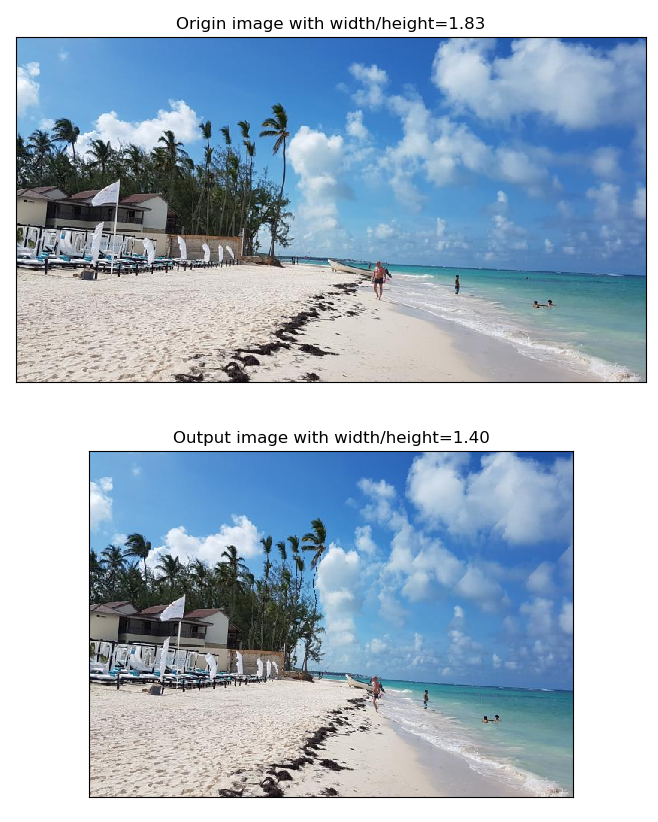
\includegraphics[width=0.8\textwidth]{../output1.png}
		\caption{Aspect Ratio Change}
		\label{Fig.output1}
	\end{figure}

	\hyperref[Fig.output1]{Figure 1}中上图为原图,宽长比为$1.83$,下图将其改为了$1.40$。可见Aspect Ratio Change后的图较好地保留了原图中能量较高的信息,同时压缩了图片的宽度。
	
	\section{Object Removal and Image Enlarging}
	核心代码和Aspect Ration Change有很多重合,这部分不再详写。
	
	此外,在实验中发现使用seam的$k$个全局最小会使得低能量seam密集的区域产生拉伸感的artifact,所以在取seam时限定了第$i$个seam的终点和第$i+1$个seam的终点之间的间距要大于$2i$,否则第$i$个seam往后顺延直到第$i^{'}$个seam的终点和第$i^{'}+1$个seam的终点之间的间距大于$2i$。
	\subsection{Procedure}
	\begin{breakablealgorithm}
		\caption{Aspect Ration Change}
		\begin{algorithmic}[1]
			
			\State Object remove
			\While{$\exists$ labeled piexl $\in$ I}
			\State Get next labeled piexl to remove from up to bottom, left to right
			\State Compute energy the same as Algorithm1
			\State Compute dp the same as Algorithm1
			\State Compute trace above p(i, :) and below p(i, :) respectively to get a seam through the pixel
			\State Remove seam form $I$ accroding to trace
			\EndWhile
			
			\State Image Enlarging
			\State Compute energy the same as Algorithm1
			\State Compute dp the same as Algorithm1
			\State Compute first $k$ seam, in which $k$ euqals to the difference between width of input image and image after removal
			\State Duplicate all of seams to the right side of origin seams given by last step
		\end{algorithmic}
		
	\end{breakablealgorithm}
	\subsection{Result}
	
	\begin{figure}[htbp]
		\centering
		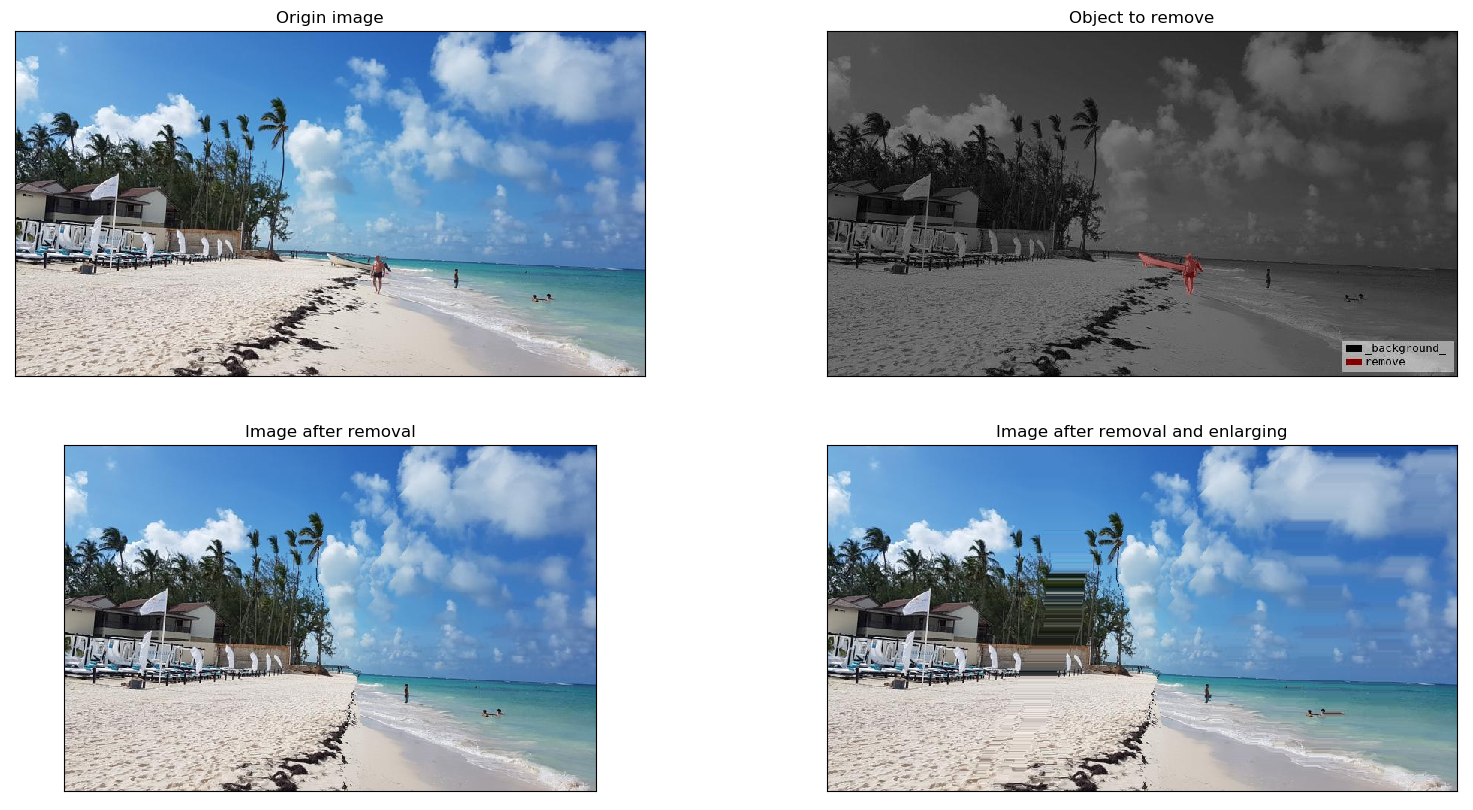
\includegraphics[width=1.0\textwidth]{../output2.png}
		\caption{Object Removal and Image Enlarging}
		\label{Fig.output2}
	\end{figure}
	
	\hyperref[Fig.output2]{Figure 2}中左上为原图,右上拿labelme标出了需要被移除的物体——人和他后面的船,左下是移除指定物体后的结果,右下是在左下的基础上做Image Enlarging恢复到原图尺寸的结果。从左下图可见Object Removal后的图完整地移除了指定的物体且较好地保留了原图中其他部分的空间结构,从右下图可见Image Enlarging后的图恢复到了原图尺寸且对能量较小的seam做了复制,但是左中部还是有较为明显的artifacts。
	
	其原因在于图左中部树林部分像素值很相近,图像梯度小,能量小。从图像底部开始做Backtracing时,很大范围内seam的路径走到图像中部都会经过这块绿色的低能量区域,造成这个区域被重复复制,进而产生拉伸感的artifacts。解决方案可以尝试从图像y轴的中部作为Backtracing的起点,然后向上下两侧分别做Backtracing和Forwardtracing找到seam.
	
	\section{Conclusion}
	这次作业加深了我对于传统Image Resize和Content-Aware Image Resizing的理解,动手实现Aspect Ratio Change, Object Remove和Image Enlarging的过程则让我对于numpy的使用变得更加熟练。
	
\end{document}